\documentclass{beamer}   % [notes=show,handout]

\usepackage{tikz}
\usepackage{graphicx}
\usepackage{hyperref}
\mode<presentation>

\usetheme{Frankfurt}%
\usecolortheme{seagull}

\definecolor{garnet}{RGB}{136,0,0}
\definecolor{clarksonGreen}{RGB}{0,52,21}

\setbeamercolor{palette primary}{fg=garnet,bg=white}
\setbeamercolor{palette secondary}{fg=clarksonGreen,bg=white}
\setbeamercolor{palette tertiary}{fg=clarksonGreen,bg=white}
\setbeamercolor{palette quaternary}{bg=clarksonGreen,fg=white}
\setbeamercolor{block title}{fg=black,bg=black!15}
\setbeamercolor{block body}{fg=black,bg=black!10}
\setbeamercolor{titlelike}{bg=garnet,fg=white} % parent=palette quaternar

\setbeamertemplate{footline}{\hspace*{.5cm}\scriptsize{\insertauthor
\hspace*{50pt} \hfill\insertframenumber\text{/}\inserttotalframenumber\hspace*{.5cm}}}

\newcommand{\R}{\mathbb{R}}


\begin{document}



\part{Introduction}
\lecture{Introduction}{Introduction}


\title{Modeling Human and Deer Interaction}
\subtitle{Actuarial Considerations}

\author{Liu, Sweeney, Zhou}
\institute{SUNY Potsdam and Clarkson University REU \\ with Dr. Kelly Black}
\date{July 30, 2013}

\begin{frame}[plain]
  \titlepage
  \begin{center}
  
\includegraphics[width=0.2\textwidth]{SUNYPotsdam}
  
\includegraphics[width=0.1\textwidth]{nsf_logobig}
  
\includegraphics[width=0.15\textwidth]{clarksonGreen}
\end{center}
\end{frame}

\begin{frame}
  \frametitle{Outline}
  \vspace{-5mm}
  \tableofcontents[]
\end{frame}



\section{Introduction}

\begin{frame}
    \frametitle{Background}
In the U.S., between July 1, 2011 and June 30, 2012:
    \begin{itemize}
    	\item 1.23 million deer-vehicle collisions occurred.
    	\item Costs are more than \$4 billion in vehicle damage.
    	\item The average claim for deer-vehicle collisions was \$3,305 per accident.
    	\item The Insurance Institute for Highway Safety (IIHS) noted that deer-vehicle collisions in the U.S. cause about 200 fatalities annually.
    \end{itemize}
\emph{(State Farm, Insurance Journal)}
\end{frame}


\begin{frame}
    \frametitle{Question?}
How do insurance companies manage funds associated with deer vehicle collisions?
\end{frame}


\section{Population Biology}

\begin{frame}
    \frametitle{Deer Population}
    \begin{itemize}
    	\item Assumptions
		\begin{itemize}
    		\item Population is near carrying capacity.
    		\item The only predation is human i.e. hunting and car fatalities.
    		\item Migrations rates are balanced across counties.
		\item Customers of one insurance company experience the same collision rate as the general population.
    		\end{itemize}
    \end{itemize}
\end{frame}

\begin{frame}
    \frametitle{Logistic Equation with Harvest}
	\vspace{-1cm}
	\begin{eqnarray*}
		\frac{dx}{dt} &=& rx \left( 1-\frac{x}{f} \right) -hx
	\end{eqnarray*}
	\begin{itemize}
		\item $f$ - Carrying capacity
		\item $r$ - Growth rate
		\item $h$ - Harvest rate
	\end{itemize}
\end{frame}

\begin{frame}
    \frametitle{Rescaling the Logistic Equation with Harvest}
	\vspace{-1cm}
	\begin{eqnarray*}
		\frac{dx}{dt} &=& rx \left( 1-\frac{x}{f} \right) -hx\\
		 &=& rx-\frac{rx^{2}}{f}-hx\\
		 &=& (r-h)x-\frac{rx^{2}}{f}\\
		 &=& (r-h)x \left(1-\frac{rx^{2}}{f(r-h)} \right)\\
		 &=& \tilde{r}x \left( 1-\frac{x}{\tilde{f}} \right)		
	\end{eqnarray*}
\end{frame}

\begin{frame}
    \frametitle{Athens County, Ohio}
Schwabe, \emph{et al.}, 2000
	\begin{itemize}
		\item Carrying capacity is approximately 28,000
		\item Growth rate is 1.7
		\item Harvest rate is 0.16
	\end{itemize}
\end{frame}






\section{Insurance}

\begin{frame}
    \frametitle{State Regulations and Bond Funds}
%%%%%%%%%%%%% How insurance companies work
	\begin{itemize}
		\item Low risk government bonds
		\item Premiums from customers
		%%%%% AREA WHERE YOU LIVE AKA DEER, driving record, age, type of car
		\item Claims based on accidents
	\end{itemize}
\end{frame}


\section{Model}

\begin{frame}
    \frametitle{Stochastics}
	\begin{itemize}
		\item Brownian Motion (Random Walks) - $W(t)$
		\item Properties
	\begin{enumerate}[i]
		\item $W(t)$ is continuous
		\item $W(t)$ is no where differentiable
		\item If $t_{1}<t_{2}<t_{3}<t_{4}$, \\
			$W(t_{1}), W(t_{2})-W(t_{1}),  W(t_{3})-W(t_{4})$ are independent random variables
		\item If $0 \le s\le t$ then $W(t)-W(s) \sim N(0, t-s)$
	\end{enumerate}
		\item Gaussian White ``Noise" - $dW$
	\end{itemize}
%%%%%%%%%% Brownian Motion, Gaussian White Noise
\end{frame}



\begin{frame}
    \frametitle{Models}
	\begin{eqnarray}
		dx &=& \tilde{r} x \left( 1- \frac{x}{\tilde{f}}\right) dt +\alpha x \, dW \\
		dm &=& ( \rho m - \beta x + P) dt - \gamma x \, dW
	\end{eqnarray}
	\begin{itemize}
		\item Known Parameters - $\tilde{r}$, $\tilde{f}$, $\rho$, $\beta$
		\item Unknown Parameters - $\alpha$, $\gamma$, $P$
	\end{itemize}
\end{frame}




\section{Numerics}

\begin{frame}
   \frametitle{Approximation}
%%%%%%%%%Include figure
\vspace*{-3em}
	\begin{eqnarray*}
		dX &=& f(X) \, dt + g(X) \, dW \\
	\end{eqnarray*}
\vspace*{-3em}
	\begin{center}
		$X_{j} =$ approximation of $X(t_{j})$ \\ [20pt]
	\includegraphics[height=4cm]{approximation}
	\end{center}

\end{frame}



\begin{frame}
    \frametitle{Methods of Approximations}
	Euler-Maruyama Method - $O(\Delta t^{1})$
	\begin{eqnarray*}
		X_{j} &=& X_{j-1} + f(X_{j-1})\triangle t+ g(X_{j-1})(W(\tau_{j})-W(\tau_{j-1})) \\
		 j &=& 1,2,... ,L \\
	\end{eqnarray*}
	Milstein Method - $O(\Delta t^{1.5})$
	\begin{eqnarray*}
		X_{j} &=& X_{j-1} + \triangle tf(X_{j-1}) + g(X_{j-1})(W(\tau_{j})-W(\tau_{j-1})) 	\nonumber\\ 
		&& + \frac{1}{2} g(X_{j-1})g'(X_{j-1})((W(\tau_{j})-W(\tau_{j-1}))^{2}-\triangle t)\\
		 j &=& 1,2,... ,L \\
	\end{eqnarray*}
\end{frame}


\begin{frame}
    \frametitle{Benchmark}
	\framesubtitle{Paths}
\hspace*{-2cm}
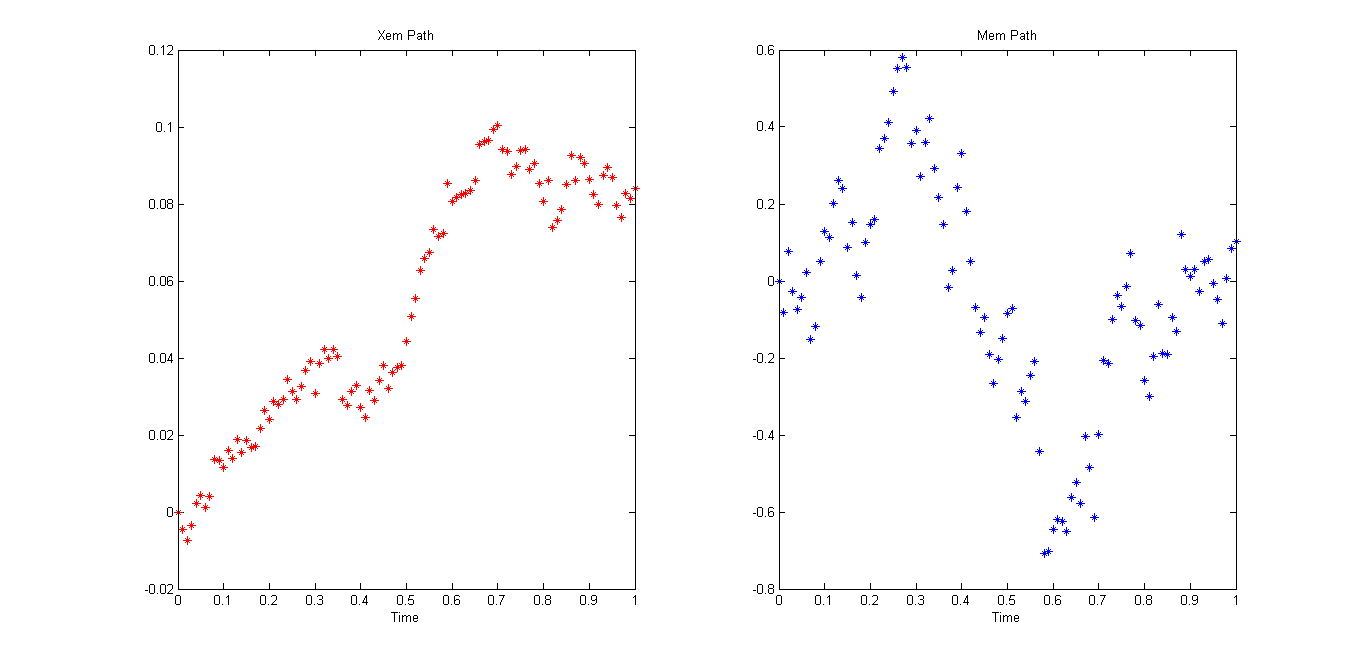
\includegraphics[height=7cm]{testpaths} 
\end{frame}


\begin{frame}
    \frametitle{Benchmark}
	\framesubtitle{Histogram}
\hspace*{-5mm}
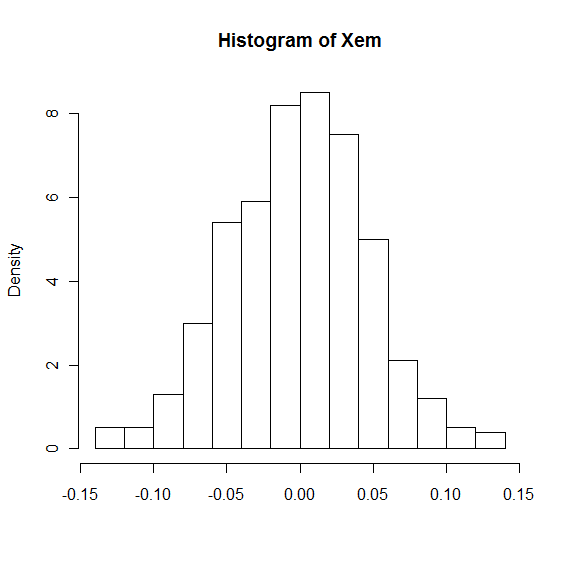
\includegraphics[height=6cm]{testhistX}
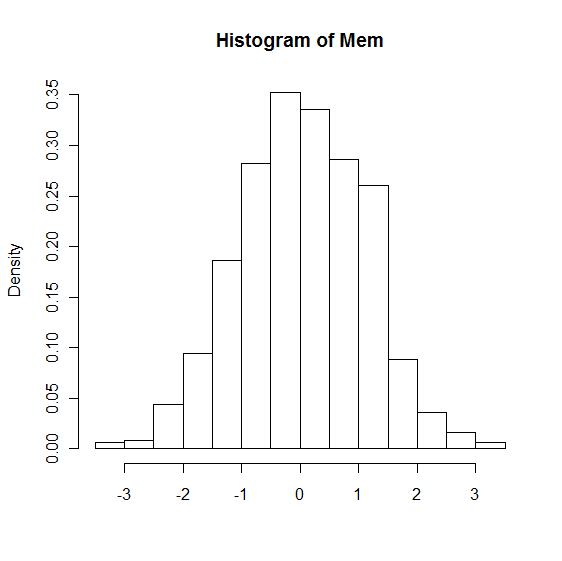
\includegraphics[height=6cm]{testhistM}
\end{frame}


\begin{frame}
    \frametitle{Benchmark}
	\framesubtitle{95\% Confidence Interval}
\begin{center}
	$\bar{x} \pm t_{(\alpha /2, df=n-1)} \frac{s}{\sqrt{n}}$ \\ 
\vspace{5mm}
\begin{tabular}{r c l c r c l}
	$E[X]$ &=& 0 && $E[M]$ &=& 0 \\
	$Var[X]$ &=& 0.0025  && $Var[M]$ &=& 1 
\end{tabular}
\end{center}
\begin{itemize}
	\item $\bar{X}$ (-0.0104, 0.00826)
	\item $\bar{M}$ (-0.172, 0.252)
\end{itemize}
\end{frame}


\begin{frame}
    \frametitle{Parameter Space}
\hspace*{-2cm}
%%%%%%%%%% Include 3D plot of parameter space
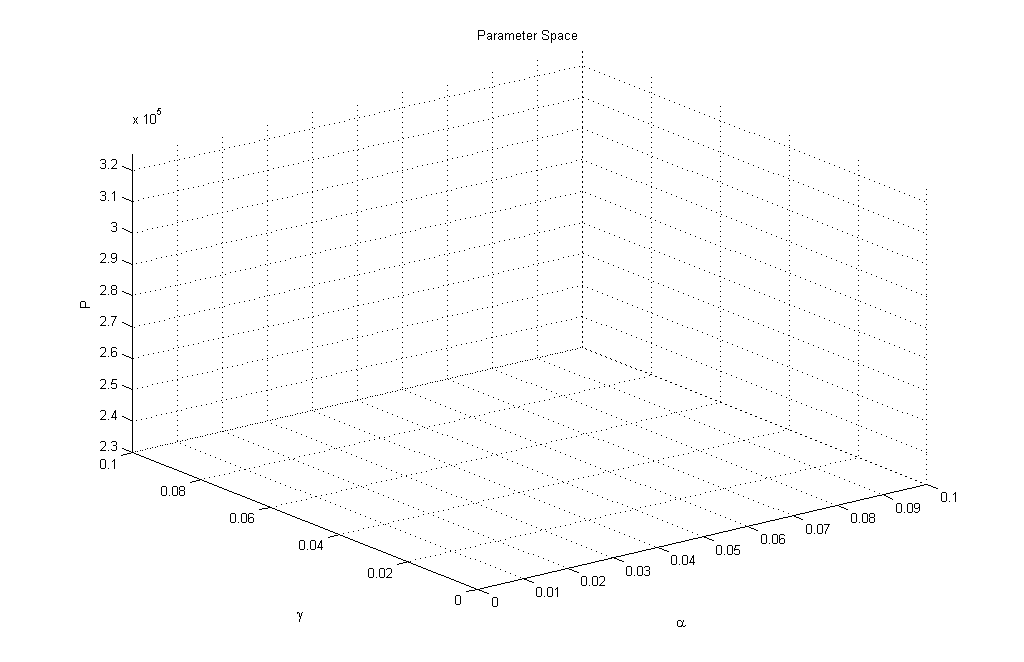
\includegraphics[height=7cm]{parameterspace}
\end{frame}









\section{Results}

\begin{frame}
    \frametitle{Results - Example for One Run}
\vspace*{-1cm}
\begin{eqnarray*}
\begin{array}{r c l r c l r c l}
	\alpha &=& .05, & \gamma &=& .05, & P &=& 230000
\end{array}
\end{eqnarray*}
\hspace*{-2cm}
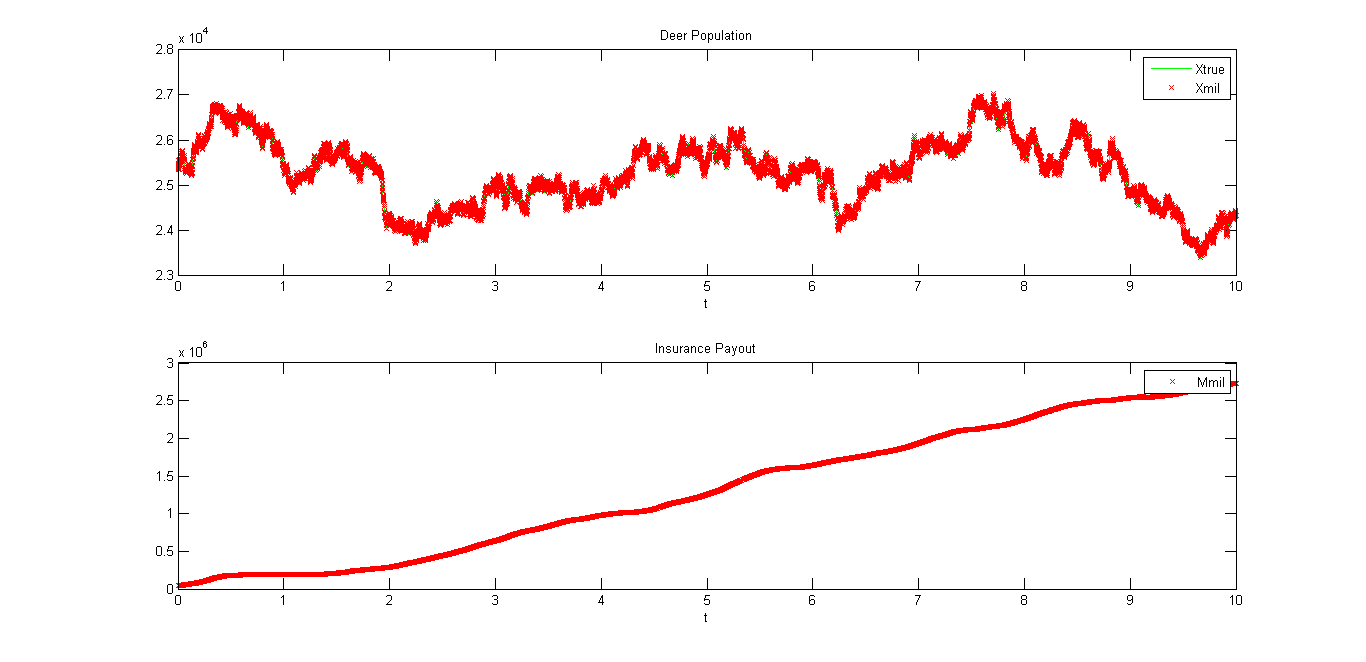
\includegraphics[height=7cm]{deerins}
\end{frame}


\begin{frame}
    \frametitle{Results - X vs. alpha }
	\framesubtitle{500 iterations}
\hspace*{-5mm}
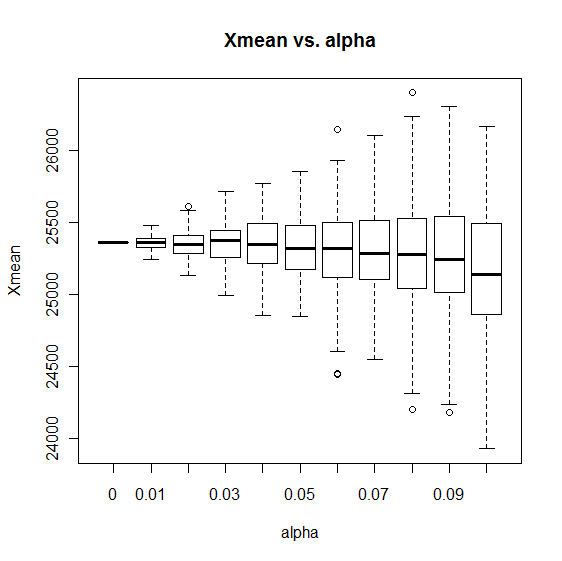
\includegraphics[height=6cm]{boxplot500_xmean_alpha}
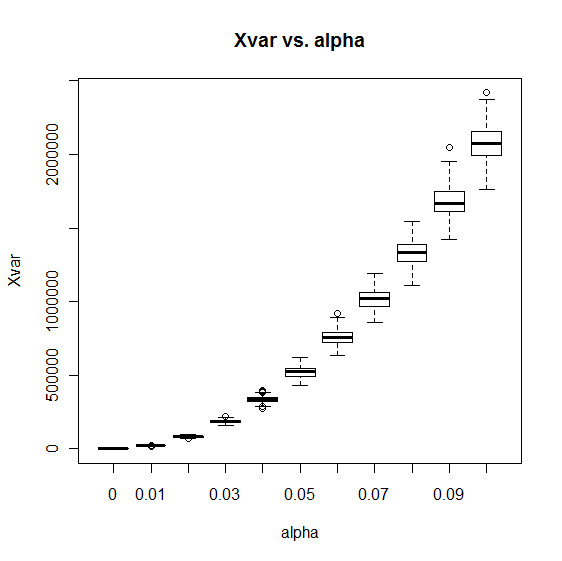
\includegraphics[height=6cm]{boxplot500_xvar_alpha}
\end{frame}

\begin{frame}
    \frametitle{Results - X vs. alpha }
	\framesubtitle{1000 iterations}
\hspace*{-5mm}
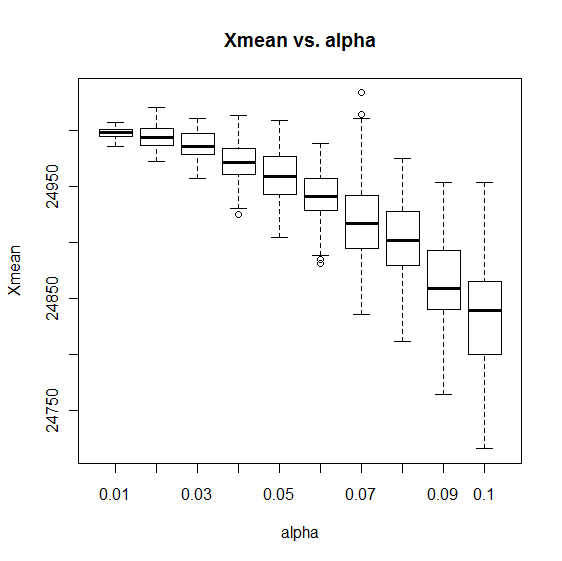
\includegraphics[height=6cm]{boxplot1000_xmean_alpha}
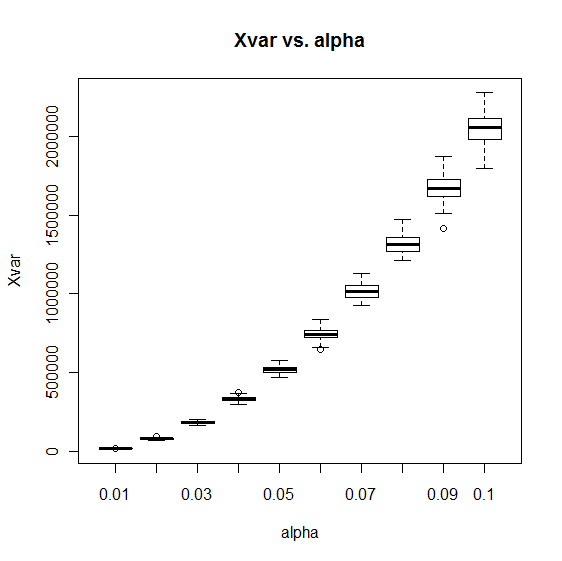
\includegraphics[height=6cm]{boxplot1000_xvar_alpha}
\end{frame}

\begin{frame}
    \frametitle{Results - Histogram}
	\framesubtitle{1000 iterations}
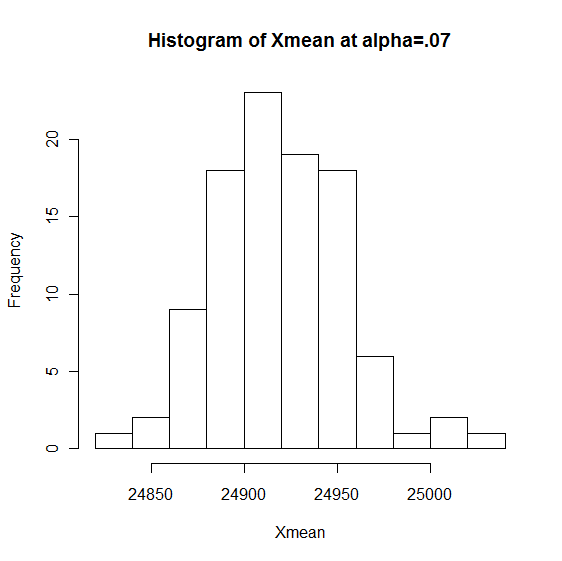
\includegraphics[height=6cm]{hist1000_xmean_alpha07}
\end{frame}



\begin{frame}
    \frametitle{Results - M vs. alpha }
	\framesubtitle{500 iterations}
\hspace*{-5mm}
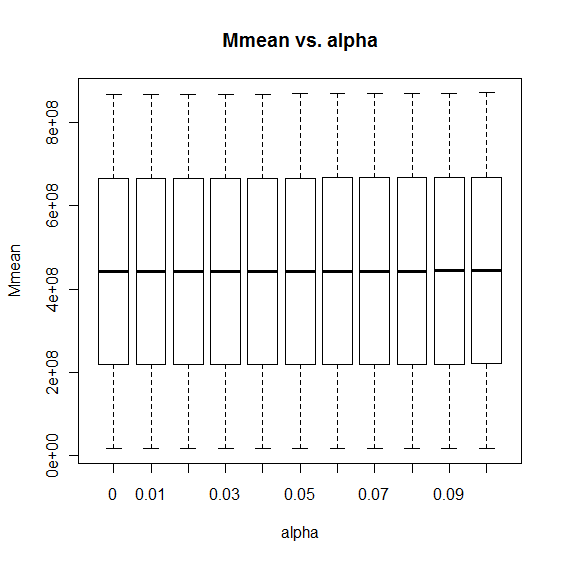
\includegraphics[height=6cm]{boxplot500_mmean_alpha}
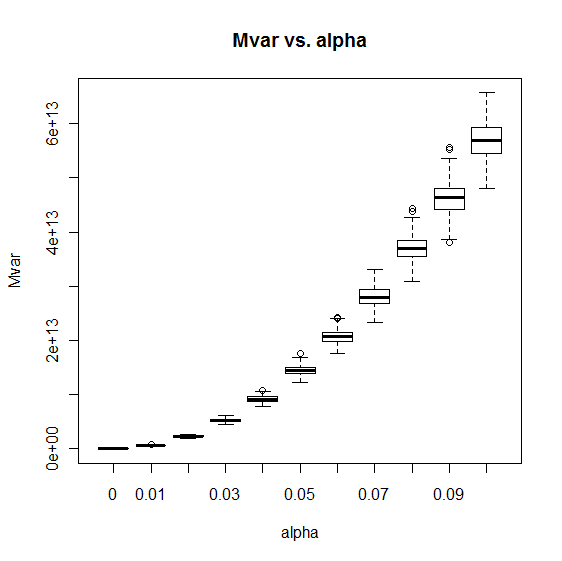
\includegraphics[height=6cm]{boxplot500_mvar_alpha}
\end{frame}

\begin{frame}
    \frametitle{Results - M vs. alpha }
	\framesubtitle{1000 iterations}
\hspace*{-5mm}
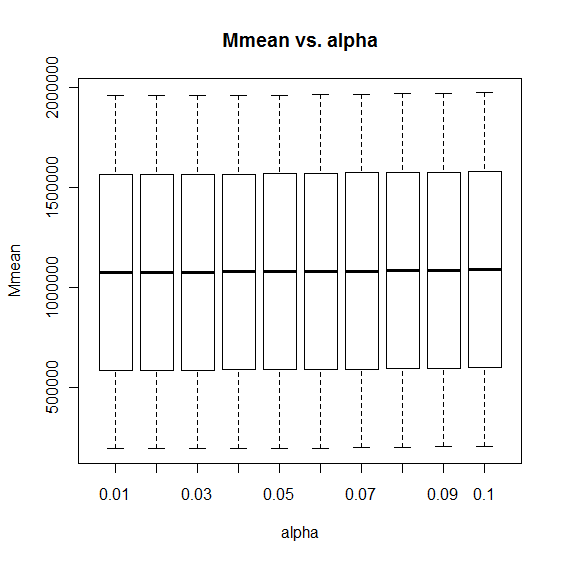
\includegraphics[height=6cm]{boxplot1000_mmean_alpha}
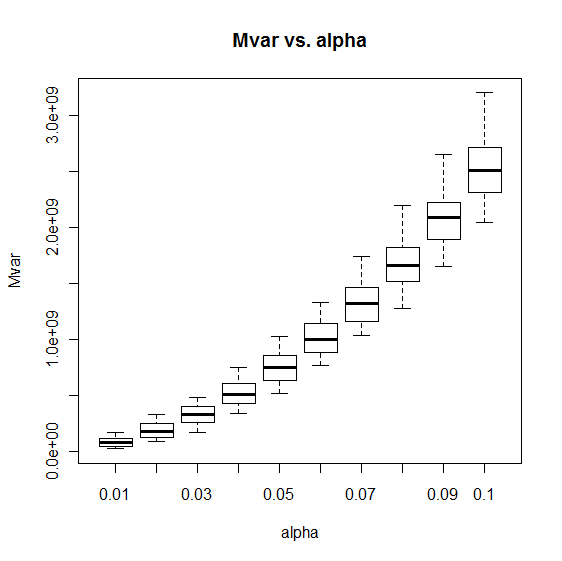
\includegraphics[height=6cm]{boxplot1000_mvar_alpha}
\end{frame}



\begin{frame}
    \frametitle{Results - M vs. gamma }
	\framesubtitle{500 iterations}
\hspace*{-5mm}
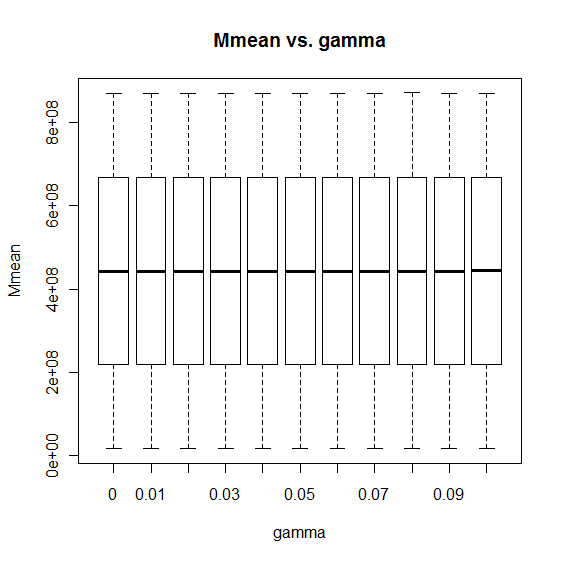
\includegraphics[height=6cm]{boxplot500_mmean_gamma}
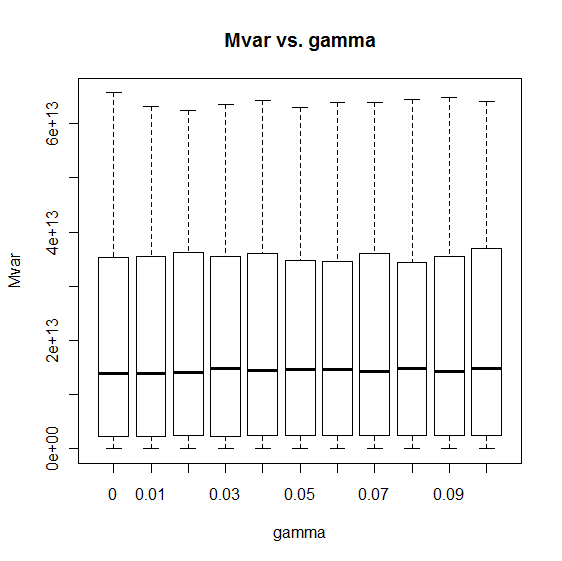
\includegraphics[height=6cm]{boxplot500_mvar_gamma}
\end{frame}

\begin{frame}
    \frametitle{Results - M vs. gamma }
	\framesubtitle{1000 iterations}
\hspace*{-5mm}
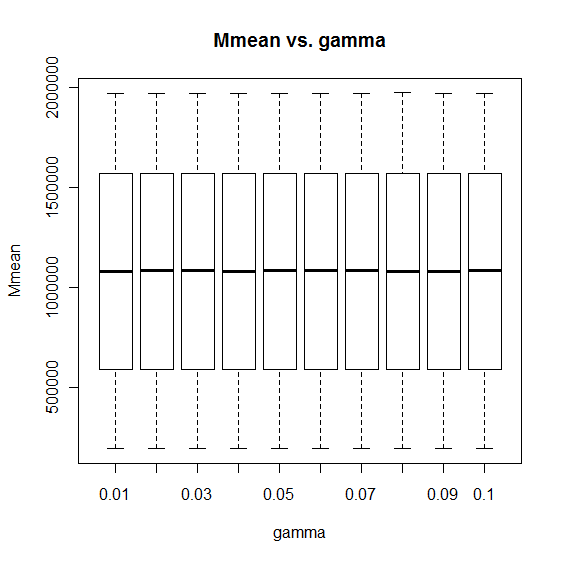
\includegraphics[height=6cm]{boxplot1000_mmean_gamma}
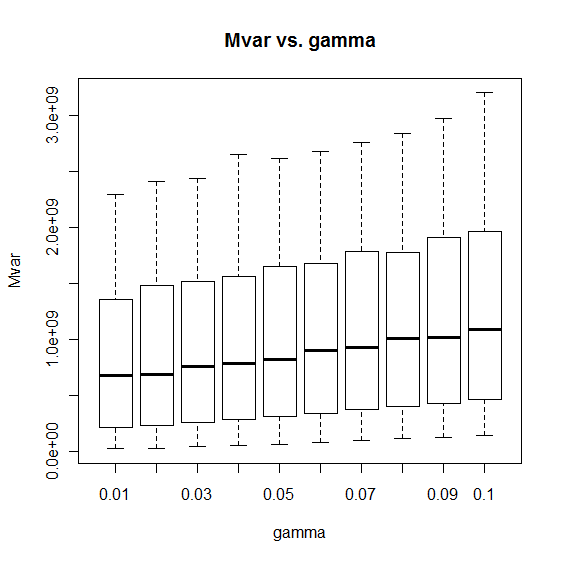
\includegraphics[height=6cm]{boxplot1000_mvar_gamma}
\end{frame}





\begin{frame}
    \frametitle{Results - M vs. P }
	\framesubtitle{500 iterations}
\hspace*{-5mm}
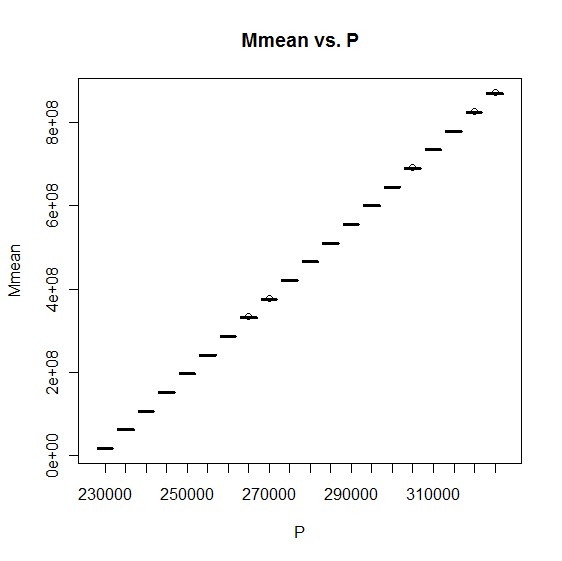
\includegraphics[height=6cm]{boxplot500_mmean_P}
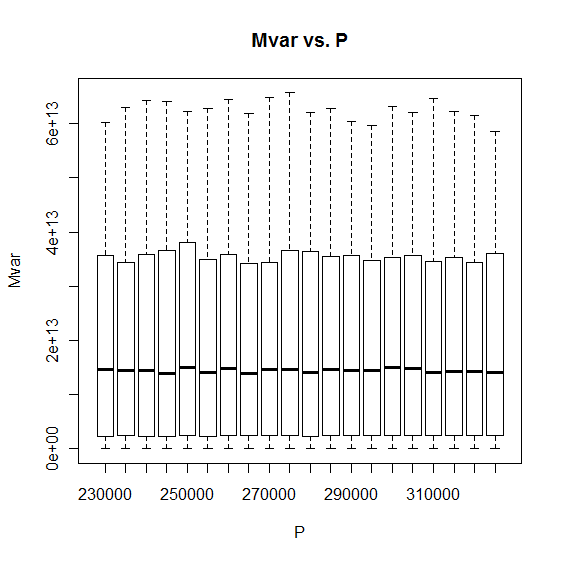
\includegraphics[height=6cm]{boxplot500_mvar_P}
\end{frame}


\begin{frame}
    \frametitle{Results - M vs. P }
	\framesubtitle{1000 iterations}
\hspace*{-5mm}
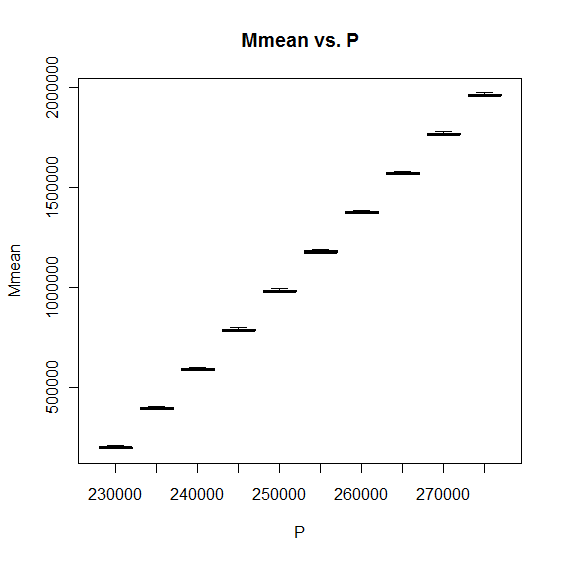
\includegraphics[height=6cm]{boxplot1000_mmean_P}
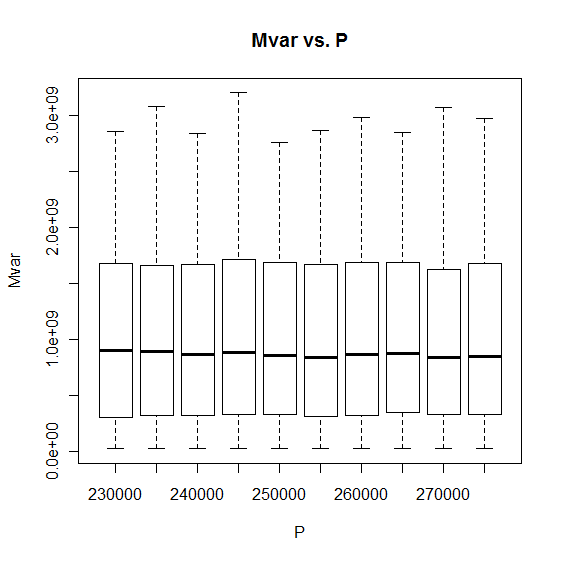
\includegraphics[height=6cm]{boxplot1000_mvar_P}
\end{frame}


\begin{frame}
    \frametitle{Video Simulations}

	\url{ https://www.youtube.com/watch?v=g-rqa3chaq8}

	\url{https://www.youtube.com/watch?v=RcQfMBF8-Og}

\end{frame}



\section{Conclusions}

\begin{frame}
    \frametitle{Conclusion}
\begin{itemize}
	\item Stochastic Model of Deer-Collisions and Insurance Bond Funds 
	\item Consistent with basic benchmarks
	\item System most sensitive to $\alpha$
	\item Linear relationship between $M$ and $P$
	\item Initial $M$ may be too big
	\item Multivariate sensitivity should be examined
\end{itemize}
\end{frame}








\section{References}

\begin{frame}
    \frametitle{References}

\begin{thebibliography}{3}

\bibitem{higham}
Higham, D. J., 2001:
An Algorithmic Introduction to Numerical Simulation of Stochastic Differential Equations.
\emph{SIAM review},
\textbf{43(3)}, 525-546.

\bibitem{schwabe}
Schwabe, K. A., Schuhmann, P. W., Tonkovich, M. J., \& Wu, E., 2000:
An Analysis of Deer-Vehicle Collisions: the Case of Ohio.
\emph{Human Conflicts with Wildlife: Economic Considerations}.

\bibitem{skiadas}
Skiadas, C. H., 2001:
Exact Solutions of Stochastic Differential Equations: Gompertz and Generalized Logistic.
\emph{Methodology and Computing in Applied Probability},
\textbf{12}, 261-270.

\end{thebibliography}

\end{frame}



\section{Acknowledgments}

\begin{frame}
    \frametitle{Acknowledgments}
	Thanks to Dr. Joel Foisy, Dr. Kelly Black and NSF (NSF \# 1262737) for their support and involvement in this program.
\end{frame}



\end{document}
